% !TEX encoding = UTF-8 Unicode

\documentclass[a4paper]{article}

\usepackage[francais]{babel}
\usepackage[T1]{fontenc}
\usepackage[utf8]{inputenc}
\usepackage{geometry}
\usepackage{graphicx}
\usepackage[colorlinks=true]{hyperref}
\usepackage{algorithm,algorithmic}
\usepackage{amssymb}
\usepackage{setspace}
\usepackage{lscape}
\usepackage{mathrsfs}
\usepackage{amsthm}
\usepackage{textcomp}
\usepackage{enumerate}

\usepackage{listings}
\usepackage{color}
\usepackage{textcomp}
\definecolor{listinggray}{gray}{0.9}
\definecolor{lbcolor}{rgb}{0.95,0.95,0.95}
\lstset{
	backgroundcolor=\color{lbcolor},
	tabsize=4,
	rulecolor=,
	language=tcl,
        basicstyle=\scriptsize,
        upquote=true,
        aboveskip={1.5\baselineskip},
        columns=fixed,
        showstringspaces=false,
        extendedchars=true,
        breaklines=true,
        prebreak = \raisebox{0ex}[0ex][0ex]{\ensuremath{\hookleftarrow}},
        frame=single,
        showtabs=false,
        showspaces=false,
        showstringspaces=false,
        identifierstyle=\ttfamily,
        keywordstyle=\color[rgb]{1,0,0},
        commentstyle=\color[rgb]{0,0,1},
        stringstyle=\color[rgb]{0.627,0.126,0.941},
}


\hypersetup{urlcolor=blue,linkcolor=black,citecolor=black,colorlinks=true}
\geometry{a4paper,twoside,left=2.5cm,right=2.5cm,marginparwidth=1.2cm,marginparsep=3mm,top=2.5cm,bottom=2.5cm}
\setlength{\parskip}{5mm plus2mm minus2mm}
\lstset{language=C, showstringspaces=false, numbers=left, numberstyle=\tiny, tabsize=4}



\begin{document}
\Large
\pagenumbering{arabic}

\begin{titlepage}
\begin{flushright}
M1 Informatique MOCA
\end{flushright}
\vfill
\begin{center}
{ \huge \bfseries Service et qualité des réseaux - TP1}\\[0.5cm]
23 mars 2012\\[3cm]

\begin{minipage}[c][4cm][t]{0.4\textwidth}
\raggedright \large
\emph{Auteurs:}\\
Chloé DESDOUITS\\
Guillerme DUVILLIE
\end{minipage}
\begin{minipage}[c][4cm][t]{0.4\textwidth}
\raggedleft \large
\emph{Professeur:} \\
Anne-\'elisabeth BAERT
\end{minipage}

\vfill

\end{center}
\end{titlepage}

\normalsize

\tableofcontents
\thispagestyle{empty}
\newpage


\section{Introduction}

Le but de ce TP était de prendre en main ns-2 (logiciel de simulation de réseaux) et de réaliser différentes expériences. Nous avons tout d'abord simulé des réseaux TCP et UDP. Puis nous avons mesuré différentes grandeurs (comme le débit moyen). Enfin, nous avons joué sur les différents paramètres et observé leur impact sur le débit pratique par rapport à sa valeur théorique.

Etudions maintenant la topologie du réseau ainsi que les paramètres utilisés.



\section{Paramètres de la simulation}

Le réseau utilisé comporte deux n\oe uds : un n\oe ud source $O$ et un n\oe ud destination $D$. Ces n\oe uds sont reliés par une connexion bidirectionnelle à débit maximum de $2 Mbits/s$. Cette connexion a une latence de $20ms$. La file d'attente entre ces deux n\oe uds peut contenir jusqu'à $100$ paquets.

La première connexion que nous avons configuré est une connexion UDP. Cette connexion suit une loi exponentielle afin de s'approcher d'une loi de poisson. Les périodes d'activité durent $10ms$ tandis que celles d'inactivité durent $5ms$. Comme nous voulons avoir un débit théorique de $1Mb/s$, nous calculons le débit moyen à partir de la formule suivante : 
$$ \overline{deb} = \frac{debCrete \times ON}{ON + OFF} $$
$$ 1Mb/s = \frac{debCrete \times 10ms}{10ms + 5ms} $$
$$ debCrete = 1.5Mb/s $$
Le débit d'envoi des paquets est donc fixé à $1.5Mb/s$ pour atteindre un débit moyen théorique de $1Mb/s$.

La seconde connexion que nous avons configuré est une connexion TCP. Cette connexion doit produire un débit constant de $1Mb/s$ ; or l'intervalle d'émission des paquets est fixé à $50ms$. Nous avons donc :
$$ \overline{deb} = \frac{taillePaquet}{intervalle} $$
$$ 1Mb/s = \frac{taillePaquet}{50ms} $$
$$ taillePaquet = 1Mb/s \times 50ms $$
$$ taillePaquet = 1Mb/s \times 50 \times 10^{-3}s $$
$$ taillePaquet = 50 \times 10^{-3}Mb $$
$$ taillePaquet =  6,25 Mo $$

Nous avons également paramétré deux connexions TCP supplémentaires de la même manière. L'une a un débit constant de $1Mb/s$ et avec un intervalle d'émission de $100ms$ et les paquets font donc $12,5 Mo$ ; et l'autre à débit constant de $1Mb/s$ et avec un intervalle d'émission de $150ms$ et les paquets font donc $18,75 Mo$.



\section{Code source du script TCL}

\lstinputlisting{../tp1.tcl}


\section{Analyse et résultats}

Nous avons tout d'abord calculé le taux de pertes et le débit moyen des trois connexions.

\subsection{Taille de la fenêtre TCP}
\begin{figure}[h]
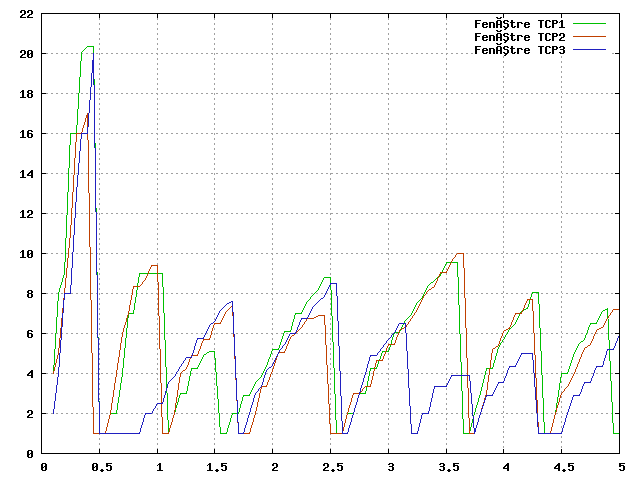
\includegraphics[width=\textwidth]{../windowSize}
\end{figure}

\subsection{Longueur de la file d'attente}
\begin{figure}[h]
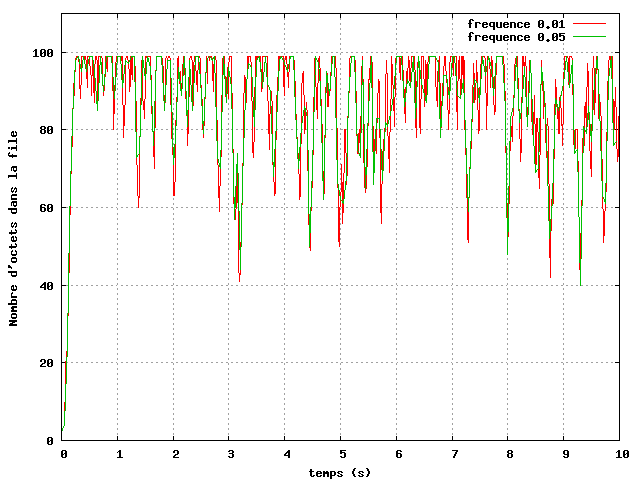
\includegraphics[width=\textwidth]{../queueSize}
\caption{Taille de la file d'attente}
\end{figure}

\vfill
{\raggedleft R\'ealis\'e avec \LaTeX{} \par}

\end{document}
